\chapter{Dataset}
\section{Struttura del dataset}
Il dataset è composto da $13$ features estratte da un set di $3762$ immagini su
scala di grigi, ciascuna immagine è stata prodotta dalla risonanza magnetica del
cervello di diversi pazienti. Di conseguenza, si hanno un totale di $3762$
istanze, ognuna etichettata con un valore categorico che rappresenta la presenza
o meno del tumore al cervello. L'etichetta è presente sotto la colonna
\textit{Class} e assume i seguenti valori:
\begin{itemize}
      \item \textbf{Presenza del tumore}: $T = 1$
      \item \textbf{Assenza del tumore}: $T = 0$
\end{itemize}

Le features vengono già date e si assumono che siano corrette rispetto alle
risonanze magnetiche del dateset\cite{explanation-features}. Più precisamente
le features si distinguono in:
\begin{enumerate}
      \item \textbf{First Order Features}: forniscono informazioni legate alle
            distribuzione dei livelli di grigio dell'immagine. Queste features
            corrispondono alle statistiche descrittive calcolate sui valori di
            ciascun pixel dell'immagine e corrispondono a:
            \begin{itemize}
                  \item \textbf{Media}
                  \item \textbf{Varianza}
                  \item \textbf{Deviazione standard}
                  \item \textbf{Indice di asimmetria}
                  \item \textbf{Indice di kurtosis}
            \end{itemize}
      \item \textbf{Second Order Features}: forniscono informazioni a livello di
            composizione della texture dell'immagine e si dividono in:
            \begin{itemize}
                  \item \textbf{Contrast}: misura la differenza tra i livelli di
                        grigio tra diverse parti dell'immagine. Maggiore sarà il
                        valore allora maggiore sarà la deviazione standard dei
                        livelli di grigio nell'immagine.
                  \item \textbf{Energy}: fornisce informazioni sulla texture e
                        sulla complessità. Maggiore sarà il valore di Energy,
                        allora maggiore sarà il contrasto oppure più dettagliata
                        sarà la texture.
                  \item \textbf{ASM}: misura quanto sono distribuiti uniformemente
                        i livelli di grigio nell'immagine. Maggiore sarà il
                        valore allora più uniforme sarà la distribuzione dei
                        livelli di grigio nell'immagine, quindi la variabilità
                        dei livelli di grigio è ridotta.
                  \item \textbf{Entropy}: misura la randomicità dei livelli di
                        grigio, quindi l'entropia sarà massima quando tutti i
                        livelli di grigio equamente probabili (randomness). Più
                        precisamente immagini con un ampio range di valori dei
                        pixel e distribuzioni uniformi di intensità tendono a
                        aumentare il valore dell'entropia.
                  \item \textbf{Homogeneous}: misura quanto sono uniformi i livelli
                        di grigio. Più alto sarà l'indice allora minore sarà il
                        contrasto dell'immagine.
                  \item \textbf{Dissimilarity}: misura quanto differiscono diverse
                        regioni dell'immagine. Un valore alto indica che si hanno
                        molte differenze tra diverse regioni della stessa immagine,
                        quindi più complessa sarà la texture.
                  \item \textbf{Correlation}: misura la correlazione dei livelli
                        di grigio tra diverse regioni della stessa immagine.
                  \item \textbf{Coarseness}: misura il grado di variazione o di
                        irregolarità dei livelli di grigio, quindi misura la finezza o
                        la granularità della texture.
            \end{itemize}
\end{enumerate}
\section{Analisi descrittiva}\label{sec:analisi-descrittiva}
Caricato il dataset, è stato eseguito un controllo per verificare che non ci fossero
valori nulli. In questo caso non sono stati trovati valori nulli, quindi non è
stato necessario eseguire alcuna operazione per la gestione di tali valori. In
secondo luogo è stato controllato se il dataset fossero presenti dei valori
duplicati e, una volta verificata la presenza si è proceduto a rimuovere un
totale di $63$ duplicati.

Successivamente, è stato eseguito un controllo sulla suddivisione degli esempi
in base alla classe di appartenenza. In particolare, questa operazione è stata
effettuata per verificare se il dataset fosse sbilanciato. Per fare ciò è stato
creato un istogramma che mostra la frequenza dei valori della colonna
\textit{Class} (visibile nella figura \ref{fig:dist-classi}).

\begin{figure}[!h]
      \centering
      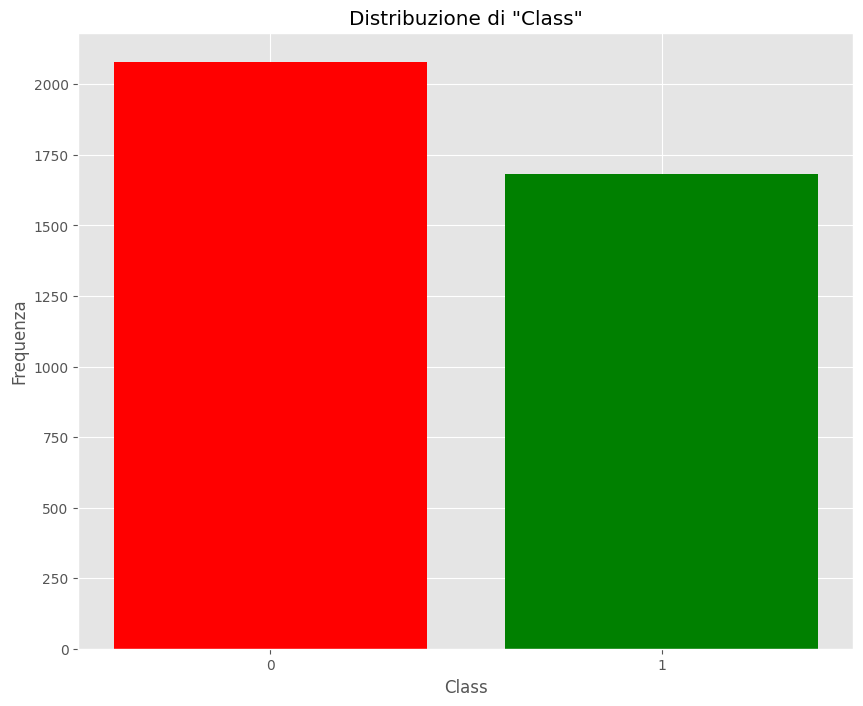
\includegraphics[width=0.5\textwidth]{img/analisi/distribuzioneClassi.png}
      \caption{Distribuzione delle classi}
      \label{fig:dist-classi}
\end{figure}

Dall'istogramma si evidenza che le classi sono abbastanza bilanciate, infatti,
il dataset è composto dal $45\%$ di esempi positivi, mentre il $55\%$ è composto
da esempi negativi.

Successivamente sono stati costruiti $13$ istogrammi, uno per ogni features
in modo tale da analizzare visivamente la loro distribuzione (i grafici sono visibili
nella figura \ref{fig:barplot_features}).

\begin{figure}[!h]
      \centering
      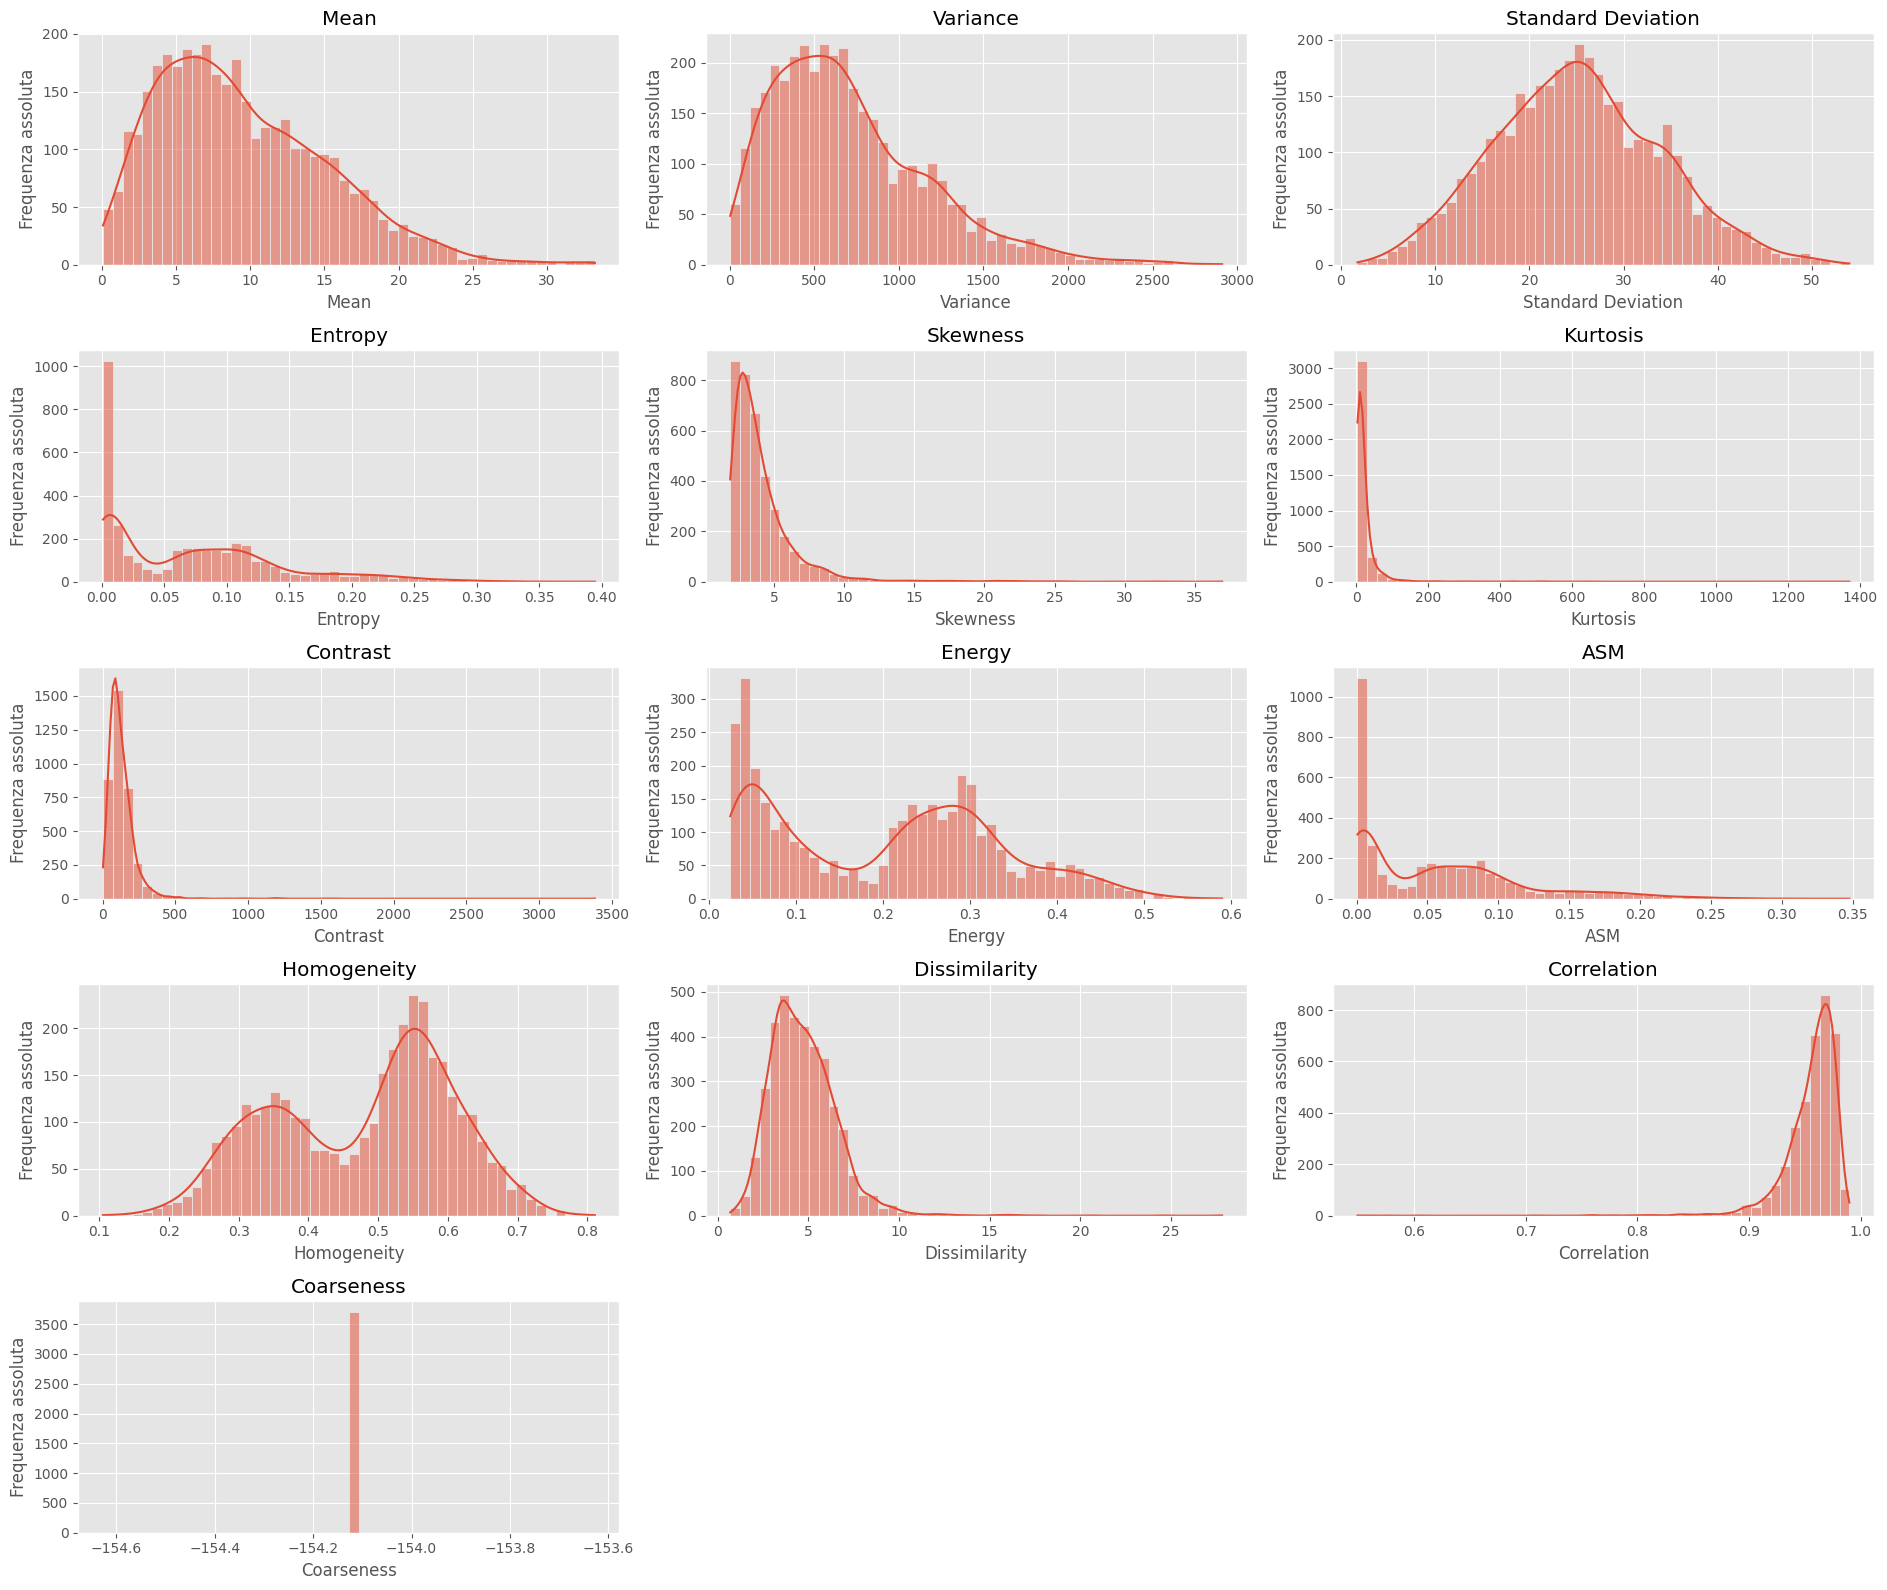
\includegraphics[width=\textwidth]{img/analisi/barplot.png}
      \caption{Barplot delle features}
      \label{fig:barplot_features}
\end{figure}

Da questi grafici si evince che le features \textit{Energy}, \textit{ASM},
\textit{Homogeneity}, \textit{Entropy} e \textit{Coarseness} non seguono una
distribuzione normale, a differenza delle altre feature che hanno un andamento
simile ad una gaussiana. In ogni caso, anche se alcune feature non seguono
l'ipotesi di normalità, si è deciso di non procedere con la loro rimozione dal
dataset ma di considerare quanto osservato nella fase di valutazione delle performance
dei modelli. In aggiunta, dal grafico si può notare che le features con una
distribuzione simile ad una normale non sono standardizzate, questa affermazione
viene anche confermata dal calcolo delle statistiche descrittive mostrate nella
tabella \ref{tab:desc-stat}.

\newpage

\begin{table}[h!]
      \begin{subtable}[h]{1\textwidth}
            \centering
            \begin{tabular}{c|c c c c c c c c c c}
                  \hline
                  \rowcolor[HTML]{EFEFEF} \cellcolor[HTML]{EFEFEF}\textbf{} & \textbf{Mean} & \textbf{Variance} & \textbf{Standard Deviation} & \cellcolor[HTML]{EFEFEF}\textbf{Entropy} & \textbf{Skewness} & \textbf{Kurtosis} \\ \hline
                  \textbf{count}                                            & 3699          & 3699              & 3699                        & 3699                                     & 3699              & 3699              \\
                  \textbf{mean}                                             & 9.473354      & 710.895793        & 25.174138                   & 0.072940                                 & 4.108362          & 24.422551         \\
                  \textbf{std}                                              & 5.732700      & 468.154274        & 8.785183                    & 0.069914                                 & 2.559163          & 56.292660         \\
                  \textbf{min}                                              & 0.078659      & 3.145628          & 1.773592                    & 0.000882                                 & 1.886014          & 3.942402          \\
                  \textbf{25\%}                                             & 4.965988      & 362.568474        & 19.041231                   & 0.006662                                 & 2.621447          & 7.265711          \\
                  \textbf{50\%}                                             & 8.468414      & 624.708056        & 24.994160                   & 0.065681                                 & 3.422625          & 12.370334         \\
                  \textbf{75\%}                                             & 13.184586     & 967.036275        & 31.097207                   & 0.112694                                 & 4.662941          & 22.760735         \\
                  \textbf{max}                                              & 33.239975     & 2910.581879       & 53.949809                   & 0.394539                                 & 36.931294         & 1371.640060       \\ \hline
            \end{tabular}
            \caption{Statistiche descrittive delle feature \textit{Mean}, \textit{Variance}, \textit{Standard Deviation}, \textit{Entropy}, \textit{Skewness} e \textit{Kurtosis}.}
            \label{tab:primameta}
      \end{subtable}
      \hfill
      \begin{subtable}[h]{1\textwidth}
            \centering
            \resizebox{0.9\textwidth}{!}{\begin{tabular}{c|c c c c c c c c}
                        \hline
                        \rowcolor[HTML]{EFEFEF} \cellcolor[HTML]{EFEFEF}\textbf{} & \textbf{Contrast} & \textbf{Energy} & \textbf{ASM} & \textbf{Homogeneity} & \textbf{Dissimilarity} & \textbf{Correlation} & \textbf{Coarseness} \\ \hline
                        \textbf{count}                                            & 3699              & 3699            & 3699         & 3699                 & 3699                   & 3699                 & 3699                \\
                        \textbf{mean}                                             & 128.119746        & 0.203546        & 0.058080     & 0.478442             & 4.702774               & 0.955697             & 7.458341e-155       \\
                        \textbf{std}                                              & 110.168137        & 0.129047        & 0.057973     & 0.127971             & 1.856688               & 0.026061             & 0.000000e+00        \\
                        \textbf{min}                                              & 3.194733          & 0.024731        & 0.000612     & 0.105490             & 0.681121               & 0.549426             & 7.458341e-155       \\
                        \textbf{25\%}                                             & 72.057782         & 0.068793        & 0.004732     & 0.364279             & 3.413266               & 0.946879             & 7.458341e-155       \\
                        \textbf{50\%}                                             & 107.075103        & 0.223482        & 0.049944     & 0.511894             & 4.486111               & 0.961567             & 7.458341e-155       \\
                        \textbf{75\%}                                             & 161.199093        & 0.298110        & 0.088870     & 0.575239             & 5.725644               & 0.971315             & 7.458341e-155       \\
                        \textbf{max}                                              & 3382.574163       & 0.589682        & 0.347725     & 0.810921             & 27.827751              & 0.989972             & 7.458341e-155       \\ \hline
                  \end{tabular}}
            \caption{Statistiche descrittive delle feature \textit{Contrast}, \textit{Energy}, \textit{ASM}, \textit{Homogeneity}, \textit{Dissimilarity}, \textit{Correlation} e \textit{Coarseness}.}
            \label{tab:secondameta}
      \end{subtable}
      \caption{Statistiche descrittive degli attributi}
      \label{tab:desc-stat}
\end{table}

Di conseguenza sarà opportuno standardizzare le features per rispettare le
assunzioni di SVM e della rete neurale. Per quanto riguarda Gaussian Naive
Bayes non è necessario effettuare l'operazione sopracitata, dal momento che nel 
calcolo della probabilità si sfrutta la formula della Gaussiana nella quale 
viene fatta una standardizzazione implicita.

Dal calcolo delle statistiche descrittive si può osservare che la feature 
\textit{Coarseness} assume un valore poco significativo tendente a $0$, quindi è 
stato pensato di convertire questa feature ad una scala logaritmica, permettendo 
di aumentare la significatività dei valori. Nonostante questa trasformazione, 
la feature presenta una deviazione standard nulla quindi questo suggerisce la 
sua esclusione dal dataset in quanto sarà quasi sicuramente una feature poco 
discriminante.

Per la fase di analisi risulta cruciale effettuare uno studio sulla potenzialità
di discriminazione dei dati. Per fare ciò sono stati prodotti un totale di $13$
grafici, uno per ogni feature, ciascuno composto da due boxplot rappresentanti
i percentili delle feature separati per le classi $0$ e $1$. I grafici sono visibili
nella figura \ref{fig:boxplot_features}.

\newpage

\begin{figure}[!h]
      \centering
      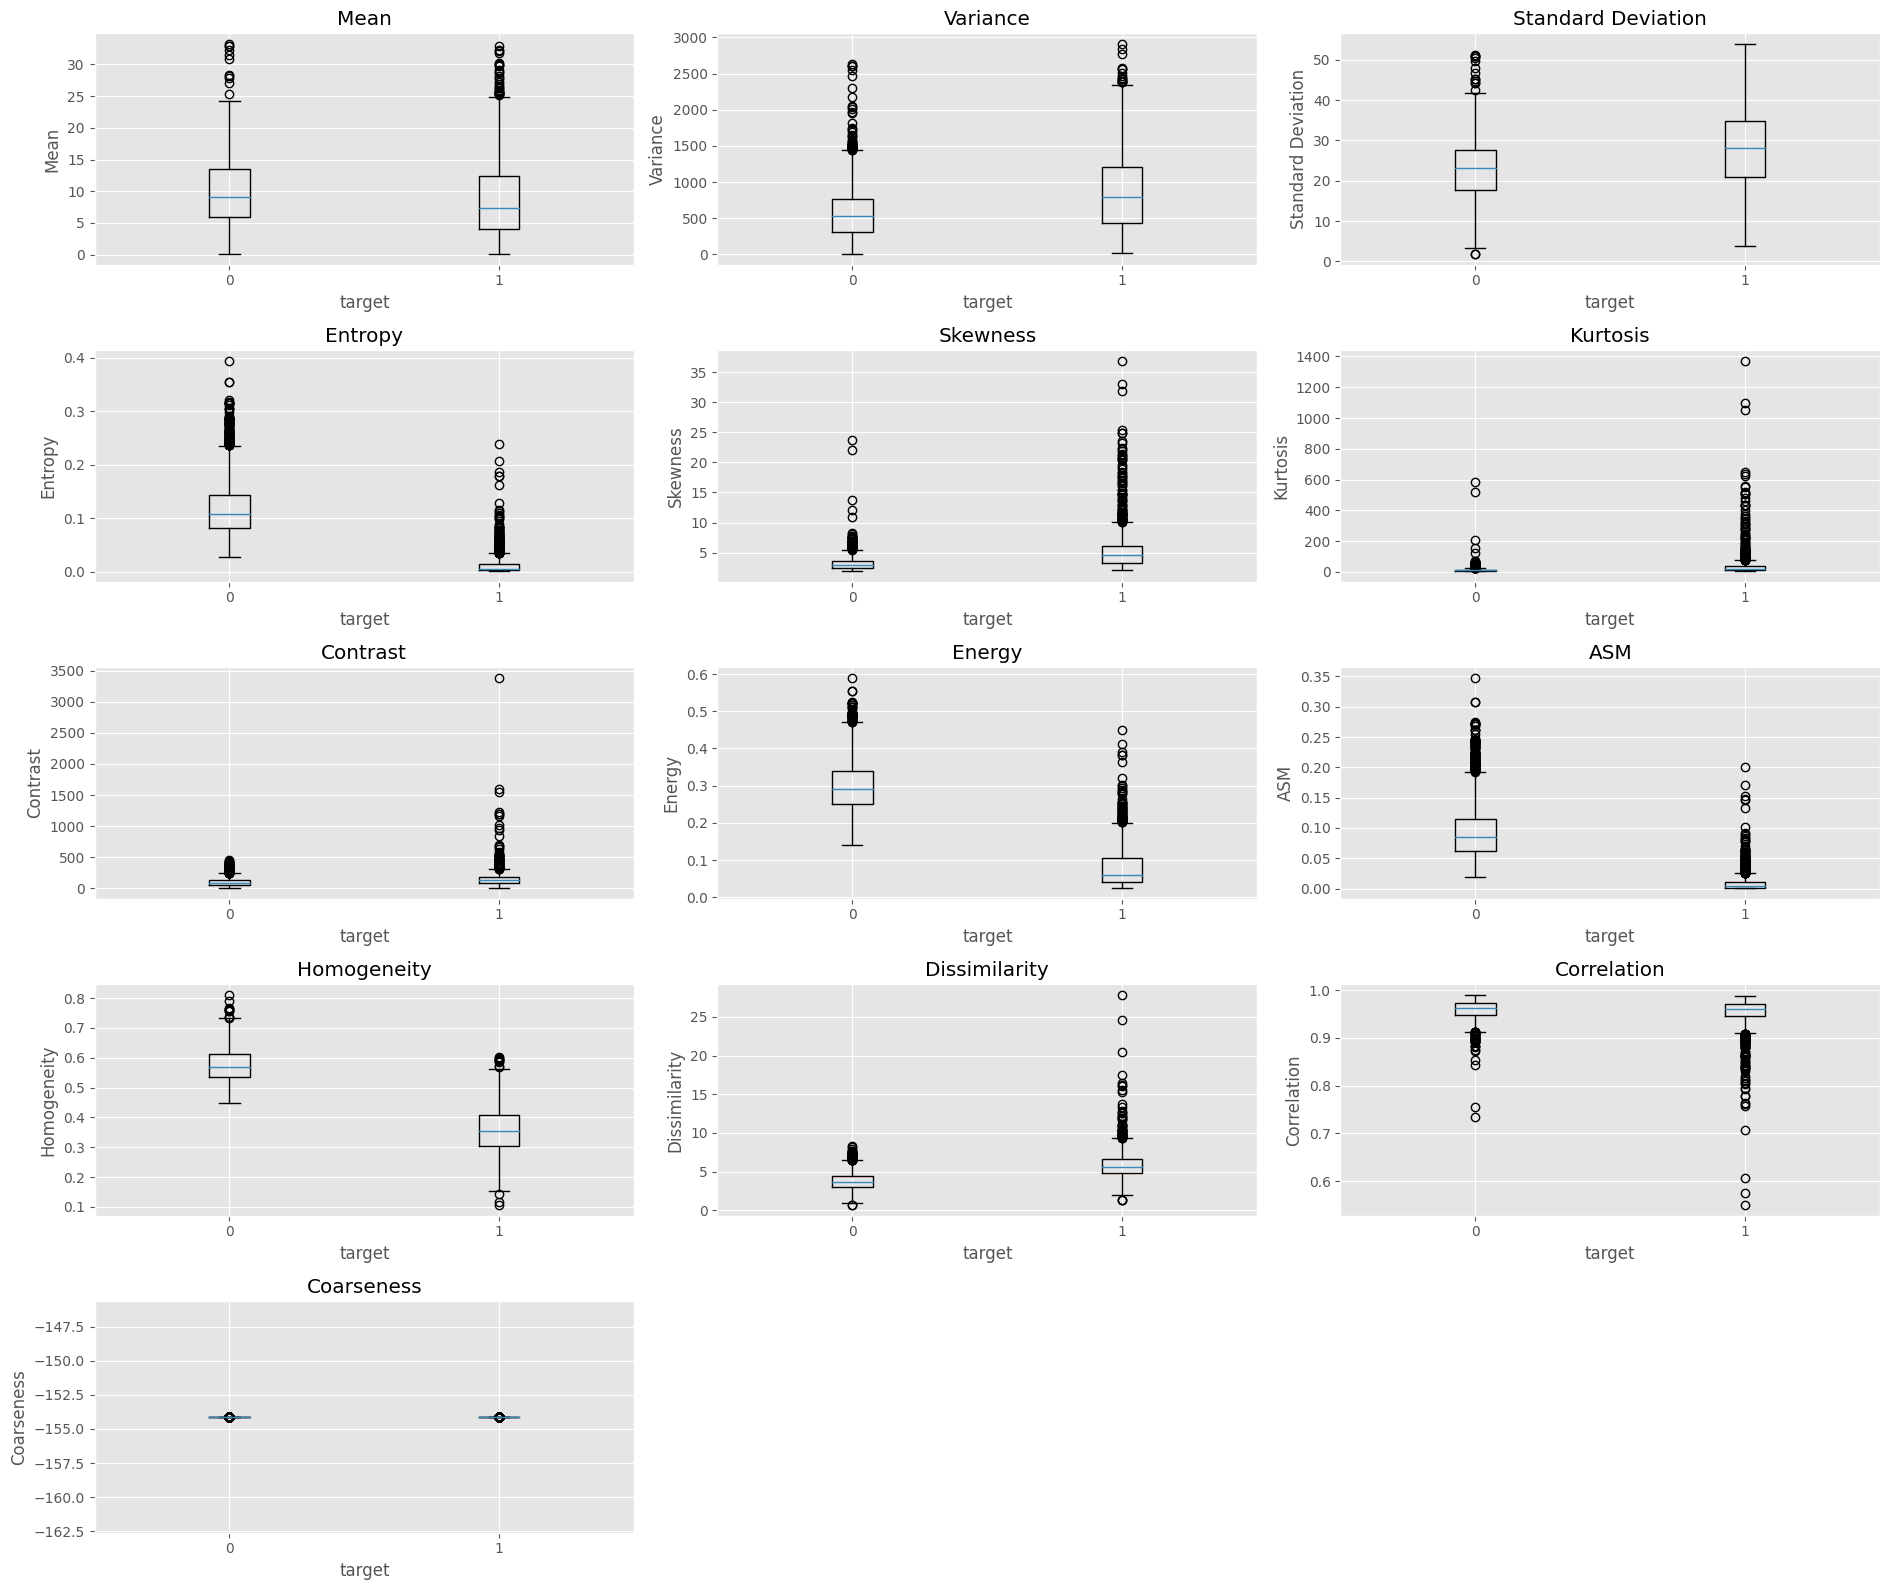
\includegraphics[width=\textwidth]{img/analisi/boxplot.png}
      \caption{Barplot delle features}
      \label{fig:boxplot_features}
\end{figure}

Dai boxplot si può osservare che nel dataset sono presenti numerosi outliers, in
aggiunta le distribuzioni delle features separate per classi si sovrappongono
quasi tutte, eccetto per \textit{Entropy}, \textit{Energy}, \textit{ASM} e
\textit{Homogeneity}. Questo implica il fatto che potenzialmente sono le più
discriminanti rispetto alle altre features. In aggiunta, i grafici confermano
che la \textit{Coarseness} è costante, quindi dal momento che non può essere un
attributo discriminate si può rimuovere dal dataset.

Infine, è stato effettuato un confronto tra features estratte 2 a 2 per poter
analizzare se le classi sono separabili linearmente considerando gruppi di due feature.
In questo modo sono state calcolate tutte le combinazioni di feature, per ogni
combinazione è stato prodotto un grafico cartesiano e un'istanza sarà disegnata
nel grafico mediante un punto. Il punto esprime $2$ informazioni:
\begin{itemize}
      \item il colore del punto specifica la classe dell'istanza
      \item le coordinate saranno i valori delle due features considerate
\end{itemize}

In aggiunta, sono stati costruiti due grafici per ogni combinazione, per identificare
quante istanze di classi diverse si sovrappongono. Tutti grafici vengono mostrati 
nella figura \ref{fig:scatterplot_features}

\newpage

\begin{figure}[!ht]
      \centering
      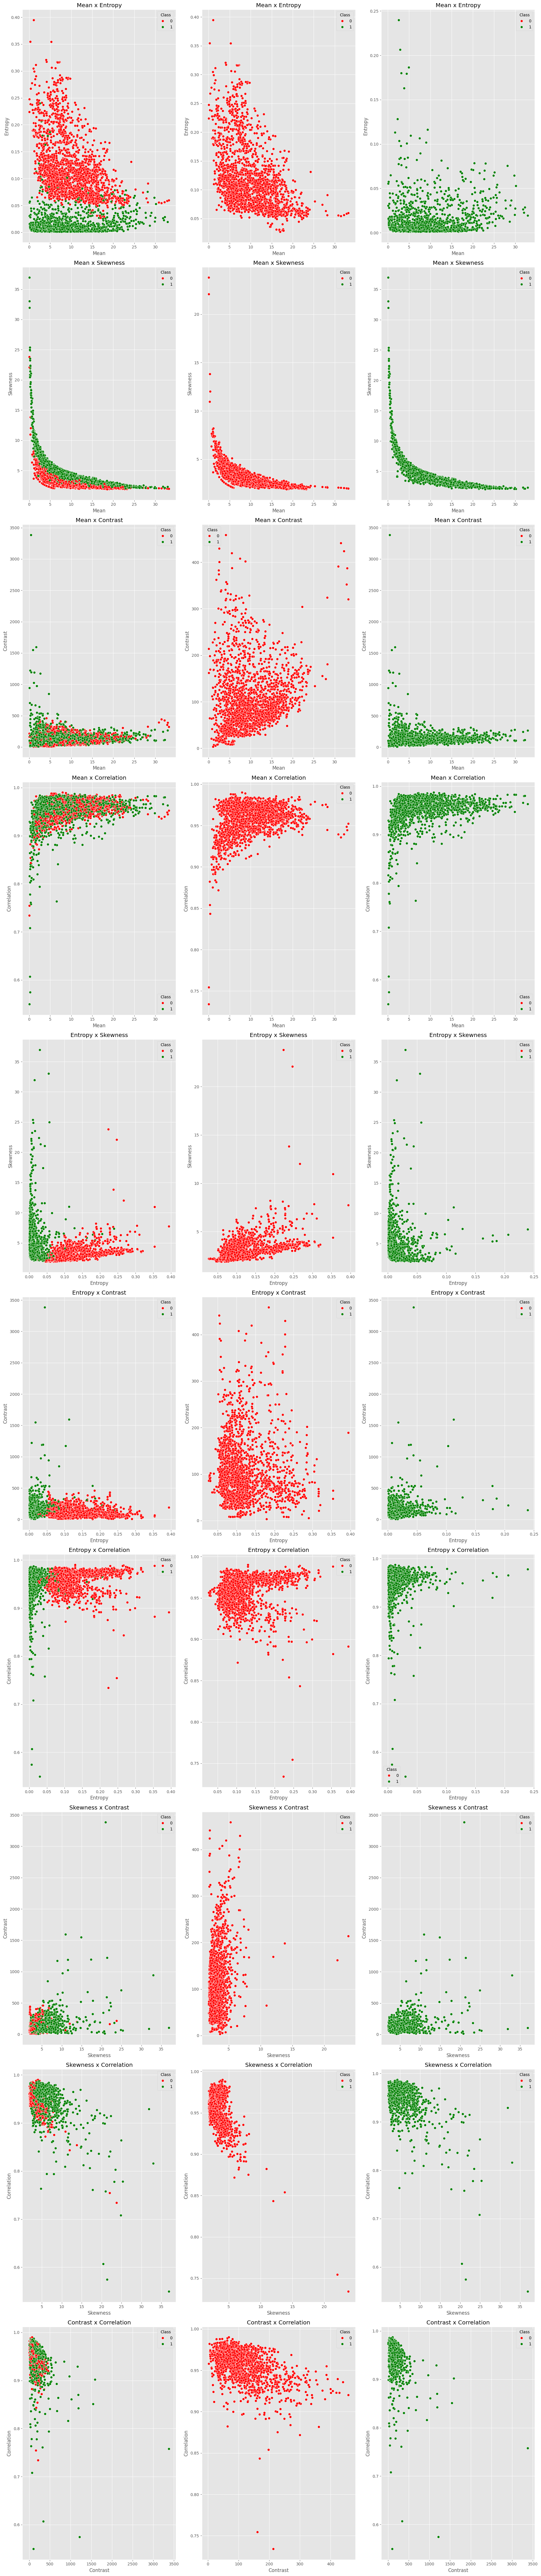
\includegraphics[height=\textheight]{img/analisi/scatterplot.png}
      \caption{Scatterplot di tutte le combinazioni di features}
      \label{fig:scatterplot_features}
\end{figure}

I grafici evidenziano il fatto che per ogni coppia di features si ha almeno una lieve sovrapposizione
delle nuvole di punti rappresentanti le due classi, questo significa che in due
dimensioni le classi non sono linearmente separabili a meno di accettare notevoli
errori. In ogni caso, si possono osservare le coppie con meno sovrapposizioni tra classi
che in questo caso sono:
\begin{itemize}
      \item \textit{Entropy} e \textit{Mean}
      \item \textit{Skewness} e \textit{Mean}
      \item \textit{Skewness} e \textit{Entropy}
      \item \textit{Contrast} e \textit{Entropy}
      \item \textit{Correlation} e \textit{Entropy}
\end{itemize}
Osservando queste coppie hanno un numero di istanze sovrapposte ridotto, allora
si può affermare che le SVM, con un kernel scelto in modo accurato, potrebbero 
ottenere degli ottimi risultati nella classificazione.
Inoltre, questi grafici permettono anticipare dei primi studi sulla correlazione
come la presenza di una correlazione logaritmica tra \textit{Skewness} e \textit{Mean}.

\subsection{Analisi delle correlazioni}
Il passaggio successivo è  stato quello di analizzare le correlazioni tra le feature
dal momento che un primo modo per ridurre la dimensionalità del dataset è attraverso
il mantenimento di solo una feature tra tutte quelle correlate.

Perciò per prima cosa è stata prodotta una matrice di correlazione, riportata in figura
\ref{fig:corr-matrix}, attraverso la quale è stato possibile osservare le correlazioni
tra le feature.

\begin{figure}[!ht]
      \centering
      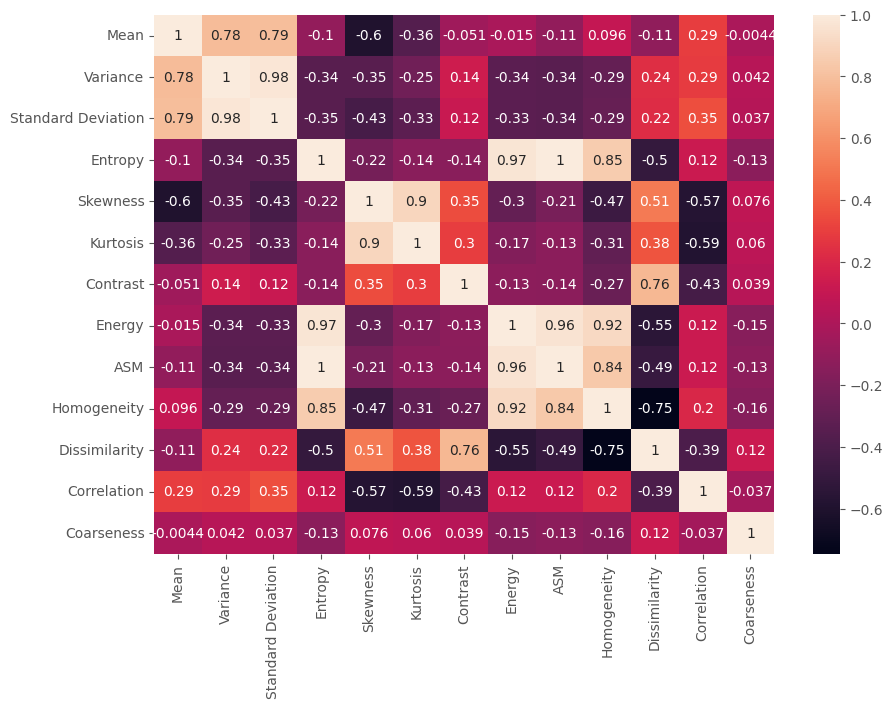
\includegraphics[width=0.5\textwidth]{img/analisi/corr.png}
      \caption{Matrice di correlazione}
      \label{fig:corr-matrix}
\end{figure}

Dall'analisi di questa matrice, si possono osservare diverse correlazioni tra le
feature. Innanzitutto, si può notare una forte correlazione positiva tra le feature
\textit{Mean}, \textit{Variance} e \textit{Standard deviation}. Questa correlazione
è facilmente spiegabile analizzando le immagini prodotte dalle risonanze magnetiche.
Infatti, essendo in bianco e nero, se la media tende a $1$ (colore bianco) allora
la varianza e la deviazione standard aumentano, perché sono presenti diversi
pixel bianchi. Questo comporta che le transizioni dal nero assoluto al bianco
assoluto necessitano di regioni di pixel maggiore rispetto ad una transizione
tra nero assoluto e grigio ($0.5$).

Invece, la correlazione tra varianza è deviazione standard facilmente spiegabile
perché la deviazione standard è la radice quadrata della varianza, quindi sono
misure dipendenti.

Una seconda forte correlazione positiva si può osservare tra le feature che
misurano l'\textbf{uniformità dei livelli di grigio} dei pixel, più precisamente
tra le feature \textit{Entropy}, \textit{ASM}, \textit{Homogeneity} ed
\textit{Energy}. Queste feature quantificano delle informazioni legate alla
texture dell'immagine, quindi la forte correlazione positiva può essere spiegata
analizzando le texture delle immagini su cui vengono calcolate. Più precisamente
se si ha un valore molto alto della feature \textit{Entropy}, significa che la
texture non è uniforme, ovvero si hanno strutture complesse e irregolari, quindi
più uniforme sarà la distribuzione dei livelli di grigio, aumentando l'indice
di \textit{ASM}, comportando di conseguenza un aumento delle variazioni di intensità
dei livelli di grigio, aumentando di conseguenza anche l'indice di \textit{Energy}
e \textit{Homogeneity}.

Al tempo stesso, la matrice di correlazione evidenza una forte correlazione positiva
tra gli indici che misurano la \textbf{morfologia della distribuzione dei livelli
      di grigio}, ovvero le feature di \textit{Skewness} e \textit{Kurtosis}. Questa dipendenza implica il
fatto che più la distribuzione è leptokurtica (Kurtosis grande), ovvero la frequenza
dei livelli di grigio dei pixel si concentrano interamente vicino alla media/mediana/
moda, allora più grande sarà la Skewness, ovvero maggiore sarà la tendenza ad avere
frequenze di livelli di grigio più vicino al bianco (coda di destra più altra rispetto
alla coda di sinistra).

La matrice della correlazione evidenzia anche una correlazione positiva tra le
feature di \textit{Contrast} e \textit{Dissimilarity}, ovvero maggiore sarà il
contrasto e maggiore sarà la complessità della texture.

In aggiunta dalla matrice si evidenza che le features di \textit{Dissimilarity}
e \textit{Homogeneity} sono correlate negativo, dal momento che misurano una dissimilarità
tra i livelli di grigio delle regioni e l'altra misura la loro l'omogeneità.

Dalla correlazione delle features è possibile ridurre la dimensionalità del dataset
considerando sono le seguenti features:
\begin{itemize}
      \item \textbf{Mean}
      \item \textbf{Entropy}
      \item \textbf{Skewness}
      \item \textbf{Contrast}
      \item \textbf{Correlation}
\end{itemize}

Per confrontare i risultati ottenuti attraverso lo studio delle correlazioni 
si è pensato di eseguire i modelli non solo sul dataset semplificato eliminando 
le correlazioni, ma anche applicando la Principal Component Analysis (PCA) per
ridurre la dimensionalità del dataset.

\section{PCA} \label{sec:pca}
Precedentemente è stato presentato un primo modo per ridurre la dimensionalità
dei dati basandoci sull'analisi delle correlazioni. In seguito, è stato pensato
di provare ad utilizzare un metodo di trasformazione delle feature per ridurre
la loro dimensionalità e successivamente analizzare i risultati ottenuti. La
scelta sul metodo da utilizzare è ricaduta su PCA.

Prima di applicare la PCA, è stato necessario standardizzare le feature, questa
operazione è stata fatta per evitare che le feature con varianza maggiore abbiano
un peso maggiore rispetto alle altre. Senza standardizzare le feature, la PCA
potrebbe non essere in grado di trovare le direzioni di massima varianza.

La prima parte dell'analisi è stata quella di trovare il corretto numero di
componenti da utilizzare per la PCA. Questo è stato fatto attraverso
l'osservazione della percentuale di varianza spiegata per ogni componente. Per
svolgere questa operazione sono state utilizzate solamente le feature numeriche
del dataset, quindi sono state escluse le colonne \textit{Image} e \textit{Class}.

Rimosse le colonne non necessarie, è stato possibile computare la PCA utilizzando
la libreria \textit{sklearn} e successivamente è stato possibile osservare la
percentuale di varianza spiegata per ogni componente, riportata in figura \ref{fig:pca}.

\begin{figure}[!ht]
      \centering
      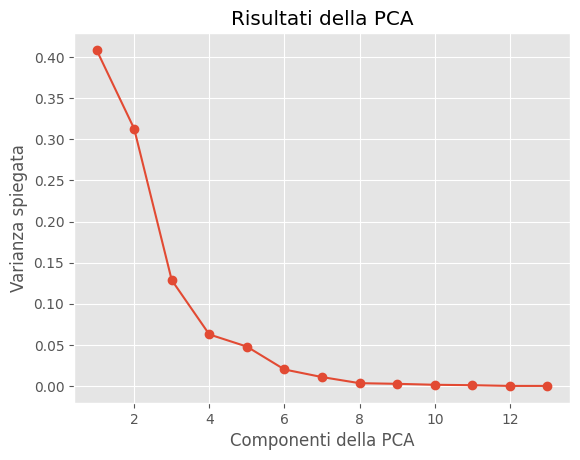
\includegraphics[width=0.45\textwidth]{img/analisi/pcaVarianza.png}
      \caption{Percentuale di varianza spiegata per ogni componente}
      \label{fig:pca}
\end{figure}

Dall'analisi della percentuale di varianza spiegata per ogni componente, si può
osservare che le prime $3$ componenti spiegano circa l'$85\%$ della varianza
dei dati. Questo ci ha permesso di ridurre la dimensionalità del dataset a soli
$3$ attributi, permettendo di rappresentare i dati in uno spazio a $3$ dimensioni.

\begin{figure}[!ht]
      \centering
      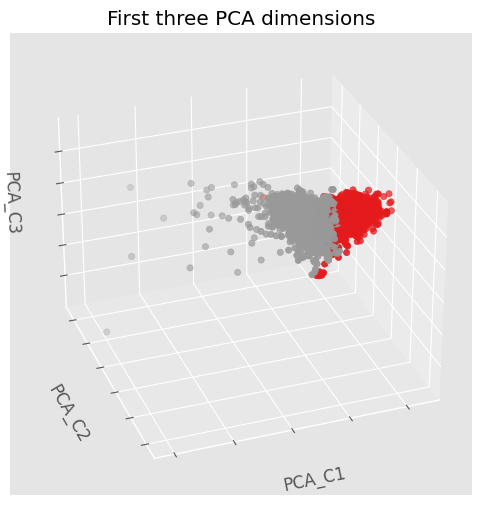
\includegraphics[width=0.4\textwidth]{img/analisi/pcaNuovoDataset.png}
      \caption{Scatter plot a 3 dimensioni}
      \label{fig:pca-3d}
\end{figure}

Dalla figura \ref{fig:pca-3d} si può osservare che i dati ottenuti dalla PCA
sembrano essere separabili con un piano.
\section{Preparazione dei dati} \label{sec:preparazione_dei_dati}
Terminata la fase di analisi dei dati, si è passati alla fase di preparazione
dei dati per l'addestramento dei modelli.

Partendo dal dataset utilizzato per l'analisi, si è proceduto con la derivazione
da esso di due dataset distinti: uno ottenuto tramite analisi esplorativa e
attraverso lo studio delle correlazioni tra gli attributi e l'altro ottenuto
tramite Principal Component Analysis (PCA).

A livello implementativo, i due dataset sono stati rinominati nel seguente modo:
\begin{itemize}
      \item \texttt{dataset\_corr}: per il dataset ottenuto tramite analisi
            esplorativa e studio delle correlazioni;
      \item \texttt{dataset\_pca}: per il dataset ottenuto tramite PCA.
      \item \texttt{dataset}: per il dataset originale.
\end{itemize}

La scelta di utilizzare due dataset distinti è stata fatta per confrontare
i due approcci e valutare quale dei due fosse più adatto per l'addestramento
dei modelli.

Ottenuti i due dataset, si è proceduto con la suddivisione di ciascuno di essi
in due sottoinsiemi: uno per l'addestramento dei modelli e l'altro per la
validazione dei modelli. Nello specifico, si è scelto di suddividere i dataset
in modo tale da avere l'$80\%$ delle istanze per l'addestramento e il $20\%$ per
il test.

La parte di dati dedicata all'addestramento dei modelli è stata utilizzata anche
per una fase di \textit{cross-validation} per la scelta dei parametri migliori
per la rete neurale e per le SVM. Per quanto riguarda la fase di ricerca degli
iperparametri migliori, si è scelto di utilizzare una k-fold cross-validation
con k=5.

La suddivisione dei dataset in training e test set è stata effettuata in modo
strutturato, ovvero mantenendo la stessa proporzione di istanze per ciascuna
classe in entrambi i set. Questo è stato fatto per evitare che i modelli
addestrati fossero influenzati da una distribuzione sbilanciata delle classi.

Infine, per la rete neurale e per la SVM, si è proceduto con la standardizzazione
dei dati, definendo due nuove varianti dei dataset \texttt{dataset\_corr} e
\texttt{dataset\_pca}:
\begin{itemize}
      \item \texttt{dataset\_corr\_std}: dataset \texttt{dataset\_corr} standardizzato;
      \item \texttt{dataset\_pca\_std}: dataset \texttt{dataset\_pca} standardizzato.
\end{itemize}

La standardizzazione dei dati è stata effettuata in quanto la rete neurale e
la SVM sono modelli che possono essere influenzati dalla distribuzione dei dati.

Nella tabella \ref{tab:riassunto_operazioni_dataset} è presentare un breve
riassunto di come sono stati preparati i dati per l'addestramento dei modelli e
quale dataset è stato utilizzato per ciascun modello.

\begin{table}[ht!]
      \resizebox{\textwidth}{!}{\begin{tabular}{@{}llc@{}}
                  \toprule
                  \rowcolor[HTML]{EFEFEF}
                  \textbf{Nome del dataset}                                                                                          &
                  \textbf{Operazioni applicate}                                                                                      &
                  \multicolumn{1}{l}{\cellcolor[HTML]{EFEFEF}\textbf{Utilizzato per i seguenti modelli}}                                                                                          \\ \midrule
                  \texttt{dataset\_corr}                                                                                             &
                  \begin{tabular}[c]{@{}l@{}}Riduzione della dimensionalità utilizzando l'analisi \\ della correlazione\end{tabular} &
                  GNB                                                                                                                                                                             \\
                  \texttt{dateset\_corr\_std}                                                                                        & dataset\_corr con la standardizzazione dei dati & SVM e NN \\
                  \texttt{dateset\_pca}                                                                                              & dataset\_corr\_std applicando l'algoritmo PCA   & GNB      \\
                  \texttt{dateset\_pca\_std}                                                                                         & dataset\_pca con la standardizzazione dei dati  & SVM e NN \\ \bottomrule
            \end{tabular}}
      \caption{Riassunto delle operazioni effettuate sui dataset e utilizzo dei dataset per i modelli.}
      \label{tab:riassunto_operazioni_dataset}
\end{table}